


\chapter{Introducing time}




\section{A new multi-structure}

In addition to the multi-structures of multi-points, multi-paths, multi-surfaces, and multi-volumes, utilizing time now introduces a new multi-structure: the {\bf multi-event}. 

An ``event" is the space-time equivalent of a point. An event is characterized by not just a position, but also by a time. In a similar manner to how copies of the same point occupying the same position creates points with different weights, multiple events occurring at the same position and time create events with different ``weights". Events with a positive weight will be commonly referred to as ``creation events", while events with a negative weight will commonly be referred to as ``destruction events". In the image below, events with a positive weight are indicated using orange dots with a ``." in the center, while events with a negative weight are indicated using purple dots with a ``X" in the center. 

\begin{center}
\begin{tabular}{cc}
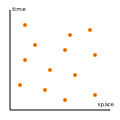
\includegraphics[width = 0.5\textwidth]{Time/multi-event_simple} & 
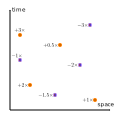
\includegraphics[width = 0.5\textwidth]{Time/multi-event_multiplicity}
\end{tabular}
\end{center}




\section{How multi-structures change with time}

This section will detail the manner in which the previously introduced multi-structures, multi-points; multi-paths; multi-surfaces; and multi-volumes, evolve with time:


\subsection{Moving points}

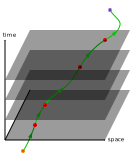
\includegraphics[width = 0.5\textwidth]{Time/world_lines}

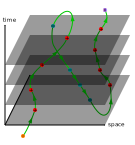
\includegraphics[width = 0.5\textwidth]{Time/world_lines_2}

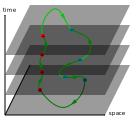
\includegraphics[width = 0.5\textwidth]{Time/world_lines_3}

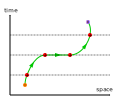
\includegraphics[width = 0.5\textwidth]{Time/infinitely_fast_point}

\begin{center}
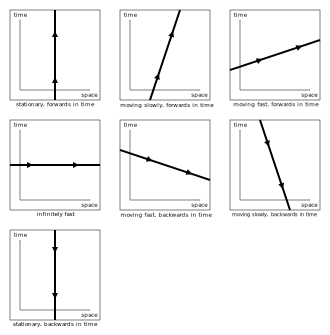
\includegraphics[width = \textwidth]{Time/world_line_interpretations}
\end{center}





\section{New intersections}  

Two new intersections will be introduced. These intersections will result in multi-events. 



\subsection{Point-surface intersections}

Given a point \(P\) with a weight of \(+1\) and an oriented surface \(\sigma\) with a weight of \(1\), then the event at which the point \(P\) passes through the surface \(\sigma\) is the intersection \(P \odot \sigma\). If \(P\) passes through \(\sigma\) in the preferred direction, then the intersection event \(P \odot \sigma\) has a weight of \(+1\). If the point \(P\) passes through the surface \(\sigma\) in the opposite direction, then the event has a weight of \(-1\). This is illustrated below:   

\begin{center}
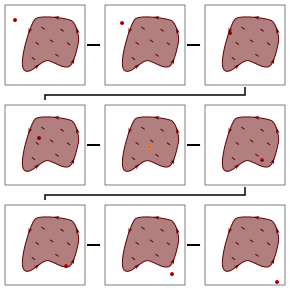
\includegraphics[width = \textwidth]{Time/point_surface_intersections}
\end{center}

With regards to notation, given a multi-point \(\rho\) and a multi-surface \(\mathbf{F}\), then the intersection will be denoted by either: 

\[\rho \odot \mathbf{F} \quad\quad\text{or}\quad\quad \mathbf{F} \odot \rho\]

Just as with path-surface intersections, a complete transit must occur for an intersection event to occur. Points that remain embedded in a surface not entering or leaving do not trigger any intersection events. As a consequence of this, given a multi-path \(\mathbf{J}\) and a multi-surface \(\mathbf{F}\), then the intersection multi-point \(\mathbf{J} \bullet \mathbf{F}\) remains embedded within the surface \(\mathbf{F}\), and no intersection events between \(\mathbf{J} \bullet \mathbf{F}\) and \(\mathbf{F}\) actually occur: 

\begin{thm}
Given multi-path \(\mathbf{J}\) and multi-surface \(\mathbf{F}\), it is the case that: 
\[(\mathbf{J} \bullet \mathbf{F}) \odot \mathbf{F} = 0\]
\end{thm}



\subsection{Path-path intersections}

Given two oriented paths \(C_1\) and \(C_2\) both with weights of \(1\), then the event at with \(C_1\) cuts through \(C_2\) is the intersection \(C_1 \otimes C_2\). Whether the intersection event has a weight of \(+1\) or \(-1\) is determined as follows: Orient your view such that \(C_1\) runs from left to right and \(C_2\) runs from bottom to top. If \(C_1\) is initially behind \(C_2\) and finishes in front of \(C_2\), then the intersection event has a weight of \(+1\). If \(C_1\) is initially in front of \(C_2\) and finishes behind \(C_2\), then the intersection event has a weight of \(-1\). This is illustrated below:    

\begin{center}
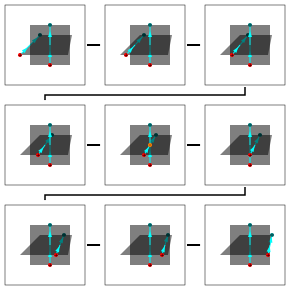
\includegraphics[width = \textwidth]{Time/path_path_intersections}
\end{center}

With regards to notation, given multi-paths \(\mathbf{J}_1\) and \(\mathbf{J}_2\), then the intersection will be denoted by: 

\[\mathbf{J}_1 \otimes \mathbf{J}_2\]  

Unlike surface-surface intersections where the ordering of the surfaces matters: \(\mathbf{F}_1 \times \mathbf{F}_2 = -(\mathbf{F}_2 \times \mathbf{F}_1)\), and that surfaces cannot intersect themselves: \(\mathbf{F} \times \mathbf{F} = 0\), the opposite is true with path-path intersections. The ordering of the paths {\bf does not} matter, and paths can in fact intersect themselves:

\begin{thm}
Given any multi-paths \(\mathbf{J}_1\) and \(\mathbf{J}_2\), it is the case that:
\[\mathbf{J}_1 \otimes \mathbf{J}_2 = \mathbf{J}_2 \otimes \mathbf{J}_1\]
\end{thm}




\subsection{Summary of intersections}

A summary of the notations used for various intersections is given below:

\vspace{5mm}

\begin{tabular}{|c||c|c|c|c|c|}
\hline
Intersections & event \(\xi_2\) & point \(\rho_2\) & path \(\mathbf{J}_2\) & surface \(\mathbf{F}_2\) & volume \(U_2\) \\
\hline
\hline
event \(\xi_1\) & 
N/A & 
N/A & 
N/A & 
N/A & 
\(\xi_1 \cdot U_2\) \\
\hline
point \(\rho_1\) & 
N/A & 
N/A & 
N/A & 
event \(\rho_1 \odot \mathbf{F}_2\) & 
point \(\rho_1 \cdot U_2\) \\ 
\hline
path \(\mathbf{J}_1\) & 
N/A & 
N/A & 
event \(\mathbf{J}_1 \otimes \mathbf{J}_2\) & 
point \(\mathbf{J}_1 \bullet \mathbf{F}_2\) & 
path \(\mathbf{J}_1 \cdot U_2\) \\ 
\hline
surface \(\mathbf{F}_1\) & 
N/A & 
event \(\mathbf{F}_1 \odot \rho_2\) &
point \(\mathbf{F}_1 \bullet \mathbf{J}_2\) & 
path \(\mathbf{F}_1 \times \mathbf{F}_2\) & 
surface \(\mathbf{F}_1 \cdot U_2\) \\ 
\hline
volume \(U_1\) & 
event \(U_1 \cdot \xi_2\) & 
point \(U_1 \cdot \rho_2\) & 
path \(U_1 \cdot \mathbf{J}_2\) & 
surface \(U_1 \cdot \mathbf{F}_2\) & 
volume \(U_1 \cdot U_2\) \\
\hline
\end{tabular}

\vspace{5mm}

%In \red{red} is indicated the ``dimensionality" of the multi-structure. Points have \(0\) dimensions; paths have \(1\) dimension; surfaces have \(2\) dimensions; and volumes have \(3\) dimensions. The number of dimensions of the intersection is the sum of the dimensions minus \(3\). When the resultant number of dimensions is less than \(0\), the intersection does not exist.



\section{Event totals}




\section{Creation/destruction events} 



A summary of the notations used for the different boundaries is given below. In addition, we have observed that the boundaries have no boundaries themselves.

\begin{center}
\begin{tabular}{|c||c|c|c|}
\hline
multi-structure & boundary & orientation & no boundary of the boundary property \\
\hline
\hline
event \(\xi\) & 
N/A & 
N/A & 
N/A \\ 
\hline 
point \(\rho\) &
event \(\nabla \odot \rho\) &
\parbox{0.25\textwidth}{
positive creation, negative destruction
} & 
\(\int (\nabla \odot \rho) = 0\) \\ 
\hline 
path \(\mathbf{J}\) & 
point \(\nabla \bullet \mathbf{J}\) & 
positive start, negative end &
\(\nabla \odot (\nabla \bullet \mathbf{J}) = 0\) \\
\hline
surface \(\mathbf{F}\) & 
path \(\nabla \times \mathbf{F}\) & 
counterclockwise &
\(\nabla \bullet (\nabla \times \mathbf{F}) = 0\) \\
\hline
volume \(U\) & 
surface \(\nabla U\) & 
inwards-oriented & 
\(\nabla \times (\nabla U) = 0\) \\
\hline
\end{tabular}
\end{center}

%In \red{red} is indicated the ``dimensionality" of the multi-structure. Points have \(0\) dimensions; paths have \(1\) dimension; surfaces have \(2\) dimensions; and volumes have \(3\) dimensions. The number of dimensions of the boundary is the number of dimensions minus \(1\). When the resultant number of dimensions is less than \(0\), the boundary does not exist.



\subsection{Balanced multi-points redefined}


Originally, the definition of a ``balanced" multi-point is a multi-point where the total point weight is \(0\). Now, a balanced multi-point is a multi-point where there are no creation or destruction events, and the world line is closed. 

A multi-point \(\rho\) is ``balanced" if and only if \(\nabla \odot \rho = 0\). 





\section{Quantification}

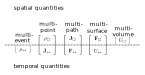
\includegraphics[width = 0.75\textwidth]{Time/quantifying_multi-structures_with_time}

\begin{itemize}
%%%%%%%%%%%%%%%%%%%%%%%%%%%%% event-volume
\item 
Multi-event: \(\xi = \left[\begin{array}{c} \hline \rho_\leftrightarrow \end{array}\right]\) and multi-volume \(U = \left[\begin{array}{c} U_\square \\ \hline \end{array} \right]\)

\[\text{Multi-event:} \;\; \xi \cdot U = \left[\begin{array}{c} \hline \rho_\leftrightarrow \end{array}\right] \cdot \left[\begin{array}{c} U_\square \\ \hline \end{array} \right] = \left[\begin{array}{c} \hline \rho_\leftrightarrow \cdot U_\square \end{array}\right]\]
%%%%%%%%%%%%%%%%%%%%%%%%%%%%% point-surface
\item 
Multi-point: \(\rho = \left[\begin{array}{c} \rho_\square \\ \hline \mathbf{J}_\leftrightarrow \end{array}\right]\) and multi-surface \(\mathbf{F} = \left[\begin{array}{c} \mathbf{F}_\square \\ \hline U_\leftrightarrow \end{array}\right]\)

\[\text{Multi-event:} \;\; \rho \odot \mathbf{F} = \left[\begin{array}{c} \rho_\square \\ \hline \mathbf{J}_\leftrightarrow \end{array}\right] \odot \left[\begin{array}{c} \mathbf{F}_\square \\ \hline U_\leftrightarrow \end{array}\right] = \left[\begin{array}{c} \hline \rho_\square \cdot U_\leftrightarrow + \mathbf{J}_\leftrightarrow \bullet \mathbf{F}_\square \end{array}\right]\]
%%%%%%%%%%%%%%%%%%%%%%%%%%%%% point-volume
\item 
Multi-point: \(\rho = \left[\begin{array}{c} \rho_\square \\ \hline \mathbf{J}_\leftrightarrow \end{array}\right]\) and multi-volume \(U = \left[\begin{array}{c} U_\square \\ \hline \end{array}\right]\)

\[\text{Multi-point:} \;\; \rho \cdot U = \left[\begin{array}{c} \rho_\square \\ \hline \mathbf{J}_\leftrightarrow \end{array}\right] \cdot \left[\begin{array}{c} U_\square \\ \hline \end{array}\right] = \left[\begin{array}{c} \rho_\square \cdot U_\square \\ \hline \mathbf{J}_\leftrightarrow \cdot U_\square \end{array}\right]\] 
%%%%%%%%%%%%%%%%%%%%%%%%%%%%% path-path 
\item 
Multi-paths: \(\mathbf{J} = \left[\begin{array}{c} \mathbf{J}_\square \\ \hline \mathbf{F}_\leftrightarrow \end{array}\right]\) and \(\mathbf{K} = \left[\begin{array}{c} \mathbf{K}_\square \\ \hline \mathbf{G}_\leftrightarrow \end{array}\right]\) 

\[\text{Multi-event:} \;\; \mathbf{J} \otimes \mathbf{K} = \left[\begin{array}{c} \mathbf{J}_\square \\ \hline \mathbf{F}_\leftrightarrow \end{array}\right] \otimes \left[\begin{array}{c} \mathbf{K}_\square \\ \hline \mathbf{G}_\leftrightarrow \end{array}\right] = \left[\begin{array}{c} \hline \mathbf{J}_\square \bullet \mathbf{G}_\leftrightarrow + \mathbf{F}_\leftrightarrow \bullet \mathbf{K}_\square \end{array}\right]\]
\end{itemize}











